%\documentclass[11pt,oneside]{Report}
%\usepackage{times}
%\usepackage{graphicx}
%\usepackage{epsfig}
%\usepackage{fullpage}
%\title{Project Viper}
%\author{Team Viper}
%\begin{document}


%\tableofcontents\newpage

%%%%%%%%%%%%%%%%%%%%%%%%%%%%%%%%%%%%%%%%%%%%%%%%%%%%%%%%%%%%%%%%%%%%%%%%%%%%%%%%%%%%%%%%%%%%%%%%%%%%%%%%%%%%%%%%%%%%%%%%%%%

\chapter{Introduction to VIPER}\label{vipintro}
% author K.Renfrew

%\textit{``A second wife is hateful to the children of the first; a \textbf{VIPER}  is not as 
%hateful''}\\
%\texttt{(Euripides, Alcestis, 438 BC.)}\\ \ \\  


%%%%%%%%%%%%%%%%%%%%%%%%%%%%%%%%%%%%%%%%%%%%%%%%%%%%%%%%%%%%%%%%%%%%%%%%%%%%%%%%%%%%%%%%%%%%%%%%%%%%%%%%%%%%%%%%%%%%%%%%%%%

\section{Rationale}
When originally developed, Vector Pascal used a command line compiler
operating in the classical Unix fashion. This interface is documented
in section \ref{commandline}.
However it has been conventional, at least since the release
of UCSD Pascal in the late '70s  for Pascal Compilers to  be provided with
an integrated development environment. The Vector Pascal IDE, provides
the usual capabilities of such environments, but with the additional feature
of   literate programming support.
%%%%%%%%%%%%%%%%%%%%%%%%%%%%%%%%%%%%%%%%%%%%%%%%%%%%%%%%%%%%%%%%%%%%%%%%%%%%%%%%%%%%%%%%%%%%%%%%%%%%%%%%%%%%%%%%%%%%%%%%%%%

\subsection{The Literate Programming Tool.}
% author K.Renfrew

Today's pace of technological development seems to be rising beyond anything that could be conceived only a few decades ago. It is a common ``joke'' that any piece of modern 
technology is six months out of date by the time it reaches the show room. 

Software development is one of the fastest moving areas of this technological stampede. With development happening at such a rate documentation is often at best a few steps 
behind the reality of the code of any system. Thus anyone attempting to maintain a system is left to their own ingenuity and some out of date documentation.

The constant updating of this documentation would in fact almost certainly be a more time consuming task than developing the program in the first place and hence time spent in 
this area can often be regarded as non productive time.

Several attempts have been made at automating this process. The automation process is often termed literate programming. The two most successful of these being 
\texttt{web} \cite{Knuth}
a development of the {\TeX} system which is the forefather of {\LaTeX}
\cite{Lamport} developed by  Leslie Lamport that is so widely used today, and JAVADOC. 
 The JAVADOC system was developed by Sun Microsystems to document programs written in JAVA by  including the document details inside specially marked comments [Sch1].      

The Vector Pascal literate programming tool will combine these two approaches by allowing the programmer to embed {\LaTeX} commands with in special comment markers. 
These will still be able to be parsed by a conventional Pascal Compiler allowing the system to be used for conventional Pascal programming.

The embedding of {\LaTeX} commands in the program is not compulsory for those wishing to use the tool.  There is a user selectable scale of detail that will be included 
automatically in documentation even from a normal Pascal program. 

In addition in an attempt to make the programs idiosyncrasies more readable and to present the programs arguments more conventionally there is the option of using a 
``mathematical syntax converter'' which will change some of the more impenetrable code into conventional mathematical symbolism 
\footnote{Refer to separate section of for the rationale of the maths syntax converter.}. The finished document being written, by the system in {\LaTeX} to allow straight 
compilation into a postscript or pdf document formats. 

To further aid the documentation the variables declared with in the program will be cross referenced to their instantiation point allowing a reader to cross reference a variable 
and thus remind themselves of it's exact nature.

This brief description clearly show the aids that a literate programming tool would bring to the programmer allowing documentation to be both kept up to date and in fact created 
retrospectively from existing code.

%%%%%%%%%%%%%%%%%%%%%%%%%%%%%%%%%%%%%%%%%%%%%%%%%%%%%%%%%%%%%%%%%%%%%%%%%%%%%%%%%%%%%%%%%%%%%%%%%%%%%%%%%%%%%%%%%%%%%%%%%%%

\subsection{The Mathematical Syntax Converter.}
% author K.Renfrew

A computer program by it's very nature has a structure which allows it to be read by a machine. Modern high level languages have abstracted themselves from this very 
successfully but never the less due to this underlying requirement the syntax of a program language can hide the program's algorithm from a human reader.

Programmers often use psuedo-code to explain algorithmic arguments. Mathematical notation is usually the most clear and precise way of presenting this argument. The 
mathematical converter allows a developer to use this system to convert the Pascal syntax into something closer to mathematical notation 
\footnote{Precise mathematical notation although perhaps desirable is a more complex operation than the time allotted to the project would allow but none the less 
an interesting development for the future.} and much more presentable to the human reader.   

This feature is unique \footnote{Unique to the best of our knowledge at the time of submission.} in a programming interface and provides a further level of documentation. 
The documentation of the algorithms involved in the program, which are arguably the program's most valuable assets.

%%%%%%%%%%%%%%%%%%%%%%%%%%%%%%%%%%%%%%%%%%%%%%%%%%%%%%%%%%%%%%%%%%%%%%%%%%%%%%%%%%%%%%%%%%%%%%%%%%%%%%%%%%%%%%%%%%%%%%%%%%%

\section{A System Overview}
% author K.Renfrew

As can be seen from the rationale above the system breaks into three main sections. The program editor with the compiler, the literate programming tool and the 
mathematical syntax converter.

It is hoped that an improvement in performance of the supplied compiler can be achieved by statically loading the compilers class files for all target processors 
\footnote{Processors currently supported are the Intel 486,Pentuin ,P3 and The Athalon K6.} at start up rather than the dynamic loading currently employed.

The I.D.E. will follow the traditional approach offering similar facilities to that of many other editors for different languages on the market place.

Among these facilities are a syntax highlighting (for Vector Pascal, {\LaTeX} and HTML), a project manager with automatic make file facility, the ability to run a program in the 
environment with redirected input and output, a function 
\& procedure finder linked to the source code, a error line highlighter for compilation errors, an external process runner for {\LaTeX} compilers, {\TeX} to HTML converters, 
a mini browser to show approximate results of the Literate programming tool etc...

The Literate programming tool has been described in it's rationale and incorporates the unique mathematical syntax conversion allowing a program to be converted to a 
mathematical argument at literally the touch of a button. 

%%%%%%%%%%%%%%%%%%%%%%%%%%%%%%%%%%%%%%%%%%%%%%%%%%%%%%%%%%%%%%%%%%%%%%%%%%%%%%%%%%%%%%%%%%%%%%%%%%%%%%%%%%%%%%%%%%%%%%%%%%%





\section{Which VIPER to download?}
%Author K.Renfrew

VIPER is  platform  independent for the operating systems it supports.
 These operating systems are: -
\begin{itemize}
\item Linux
\item Windows 9x
\item Windows NT/2000/XP
\end{itemize}

The only decision to make on the VIPER download is 
whether the source code is required. 
The source version although much larger contains the source code 
for the VIPER I.D.E. and the Vector Pascal Compiler and all 
files required for a developer to further develop or adapt any of the
 systems within VIPER. 
The class file download provides the required files to have an 
operational VIPER installation.

%%%%%%%%%%%%%%%%%%%%%%%%%%%%%%%%%%%%%%%%%%%%%%%%%%%%%%%%%%%%%%%%%%%%%%%%%%%%%%%%%%%%%%%%%%%%%%%%%%%%%%%%%%%%%%%%%%%%%%%%%%%

\section{System dependencies}
%Author K.Renfrew

 VIPER depends on several pieces of software all of 
which are freely available to download from various sources.
The vital dependencies are: -
\begin{itemize}
\item Java 1.3 or newer.
\item The NASM assembler. 
\item The gcc linker. Included in Linux installations, for Windows use the cygwin or DJGPP versions of the gcc linker.
\end{itemize}

For full functionality the following systems are also required: -
\begin{itemize}
\item A {\LaTeX}  installation. {\LaTeX} usually comes with Linux installations. The total MiK{\TeX} package is recommended for all Windows installations. 
\item A dvi viewer usually included with a {\LaTeX}  installation. The YAP viewer included with MiK{\TeX}  is particularly recommended.
\item A {\TeX} to \texttt{HTML} converter. TTH was used in the development of the system.
\end{itemize}

It is recommended that all the above programs are set-up as per their own 
installation instructions and the appropriate class path established to suit 
the host machines operating system.

%%%%%%%%%%%%%%%%%%%%%%%%%%%%%%%%%%%%%%%%%%%%%%%%%%%%%%%%%%%%%%%%%%%%%%%%%%%%%%%%%%%%%%%%%%%%%%%%%%%%%%%%%%%%%%%%%%%%%%%%%%%

\section{Installing Files}
%Author K.Renfrew

Assuming the VIPER files have been downloaded to a suitable place on the host machine the actual installation can begin. The only decision that must be made is where to install VIPER. VIPER can be installed anywhere on the host machine provided that there are no spaces in the directory path of the target directory.

Once this decision has been made the .zip file should be unzipped using a proprietary zip tool (e.g. WinZip, zip magic etc.) to the source directory.

When the .zip file has been unzipped there will be a directory called VectorPascal in the target directory. VectorPascal is the home directory of the VIPER system. 

VIPER may be launched by : -
\begin{itemize}
\item All installations. Open a shell / DOS window change to the VIPER home directory and type the command \texttt{java viper.Viper} taking care of the capital letter.
\item  Windows installations. The batch file viper.bat is included in the VIPER home directory; running this will start VIPER. A shortcut to this batch file should be placed on the host machines desktop for the easiest start-up.
\item Linux installations. The shell script viper.sh is included in the VIPER home directory; running this will start VIPER.
\end{itemize}

%%%%%%%%%%%%%%%%%%%%%%%%%%%%%%%%%%%%%%%%%%%%%%%%%%%%%%%%%%%%%%%%%%%%%%%%%%%%%%%%%%%%%%%%%%%%%%%%%%%%%%%%%%%%%%%%%%%%%%%%%%%

\section{Setting up the compiler}
%Author K.Renfrew

VIPER detects the operating system installed at start up and then moves a suitable run time library into the ../VectorPascal/ilcg/Pascal directory where it will be available for the compiler. This is done automatically each time that VIPER is started.

The compiler options will need to be set-up along with the personal set-up proffered for the installation (see Chapter \ref{userguide}). The file type for the linker will need set-up.
These options are: -
\begin{itemize}
\item For Linux or Windows using the Cygwin gcc use ``elf''.
\item For Windows using the DJGPP linker use ``coff''.
\end{itemize}

It is important to read through the user guide (see Chapter \ref{userguide}) to avoid learning the system the painful way!

%%%%%%%%%%%%%%%%%%%%%%%%%%%%%%%%%%%%%%%%%%%%%%%%%%%%%%%%%%%%%%%%%%%%%%%%%%%%%%%%%%%%%%%%%%%%%%%%%%%%%%%%%%%%%%%%%%%%%%%%%%%
  
\chapter{VIPER User Guide}{\label{userguide}

\section{Setting Up the System}
% author K.Renfrew

VIPER automatically sets the compiler flags to suit the operating system on the host machine. For those who have used the Vector Pascal 
compiler with a command line interface this means that the -U flag is set for Windows 9x and Windows NT installations, and not set for Linux/UNIX 
installations, the -o flag is set to produce an exe file with the same name as the Pascal source file. The .asm file and .o files are similarly named.
If these flags mean nothing then that is not a problem, either ignore the preceding information or see the Vector Pascal reference manual in the help files
of the VIPER system.

VIPER cannot however detect the versions of the gcc linker installed, this is left for the user. The -f flag of the compiler tells the compiler the file 
format to be used. To set this go to Set-Up / Compiler Options / Options and click the -f button and enter the file format into the adjacent text field.
The format should be :
\begin{itemize}
\item  Linux Installations and Windows installations with Cygwin gcc linker format is \texttt{elf}
\item Windows with DJGPP linker format is \texttt{coff}
\end{itemize}
\begin{figure}[h]
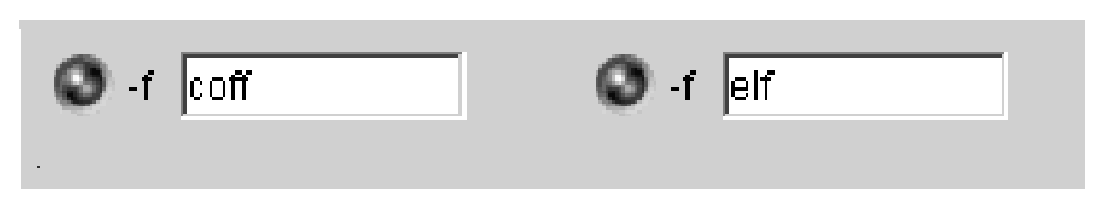
\epsfig{file=elfcoff.eps,width=2.5in}
\caption{File Format Entries in Compiler Options}\label{fig:elfcoff}
\end{figure}
 The other options on the Compiler options window are: -
 \begin{itemize}
 \item Smart (Not Yet Implemented on the V.P. compiler) Serializes / deserializes the code tree for the processor. This allows the 
compiler to `learn' how to quickly respond to a given code segment.
\item   S suppresses the assembly and linking of the program (an assembler file is still produced).
\item V causes the compiler to produce a verbose output to MyProg.lst when compiling MyProg.pas.
\item CPUtag This option is used in conjunction with the -cpu option. It prefixes the .exe file with the name of the cpu for which the 
compiler is set. when this option is used the .exe cannot be run in the I.D.E.
\item -cpu This option allow the source file to be compiled to a range of processors. To produce an exe file for a range of processors
the CPUtag should be set. This prevents the exe file being over written by the next compilation for a different processor. Subsequent 
compilations for the same processor, however, will be overwritten. Select the cpu from the list in the drop down menu adjacent to the 
-cpu button.
\item -ISO (Not Yet Implemented on the V.P. compiler) Compiles to iso standard Pascal.
\end{itemize}
\subsection{Setting System Dependencies}
VIPER depends on various other systems for full functionality. These are set in Set-Up / Compiler Options / Dependencies 
\begin{figure}[h]\center
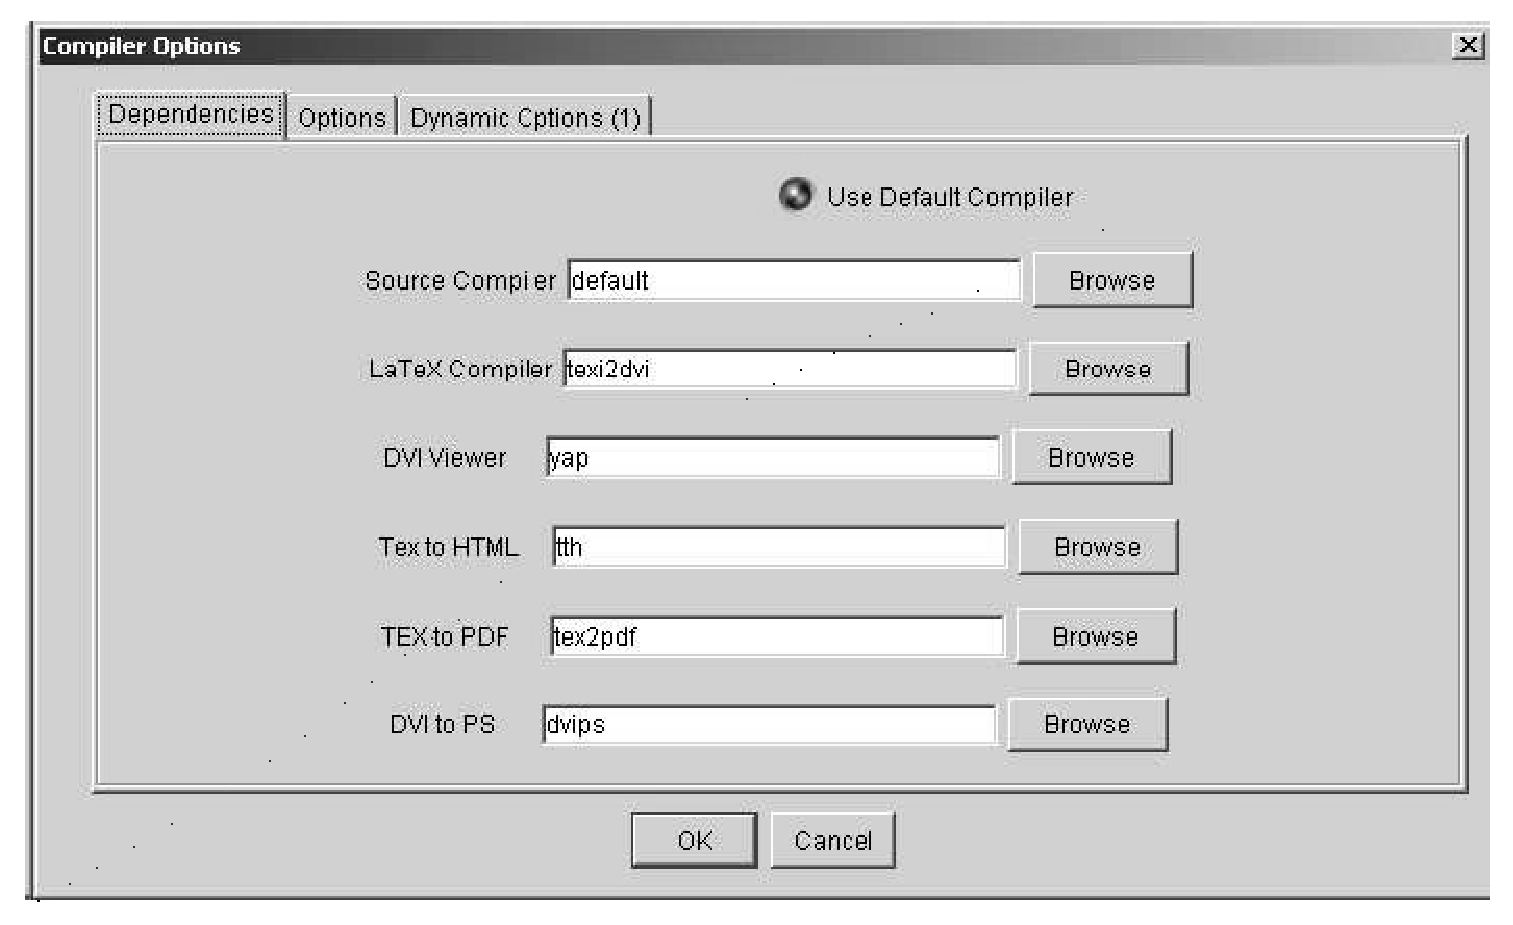
\epsfig{file=dependencies.eps,width=4.5in}
\caption{Dependencies Window}\label{fig:depnd}
\end{figure} 
The fields are: -
\begin{enumerate}
\item Source Compiler this option is only editable if the Default Compiler option is not set. This is the command that would run the compiler 
from the VectorPascal directory.
\item This is the command required to run {\LaTeX} this is required for VP{\TeX}  to work. The recommended option for this field is 
\texttt{texi2dvi}.
\item DVI viewer The dvi viewer that is to be used to view the {\LaTeX}  recommended option is YAP (Windows installations).
\item Tex to HTML if a converter is installed on the host machine then put the command in this field.
\item Tex to PDF enter the command used to convert tex to PDF.
\item DVI to PS command to convert DVI files to PostScript (usually dvips).
\end{enumerate}

%%%%%%%%%%%%%%%%%%%%%%%%%%%%%%%%%%%%%%%%%%%%%%%%%%%%%%%%%%%%%%%%%%%%%%%%%%%%%%%%%%%%%%%%%%%%%%%%%%%%%%%%%%%%%%%%%%%%%%%%%%%

\subsection{Personal Set-up}
% author K.Renfrew

Viper allows the user many options to cater for different tastes and programming styles. It is not crucial to the system to set these options but it does 
make for a more comfortable programming environment.

If your VIPER installation is on a network each user may have a different personal set-up providing each user has a separate home directory. 
VIPER installs a file called \texttt{viper.properties} into this directory and updates this file when ever a change is made to the system set-up. 

\textbf{NOTE}  The individual set-up should not be attempted when multiple files are open. If this is done then no harm comes to the system or 
any of the open files but users may experience difficulty in closing one or more files. The solution is to use Window / Close All to close all the files. 
The system can then be used as normal.
  
\subsubsection{Viper Options}
In the Set-up menu there is the Viper Options menu option. In this you will find all the familiar I.D.E. options such as font size and style, icons sizes, 
syntax colours, look and feel etc.
\begin{figure}[h]\center
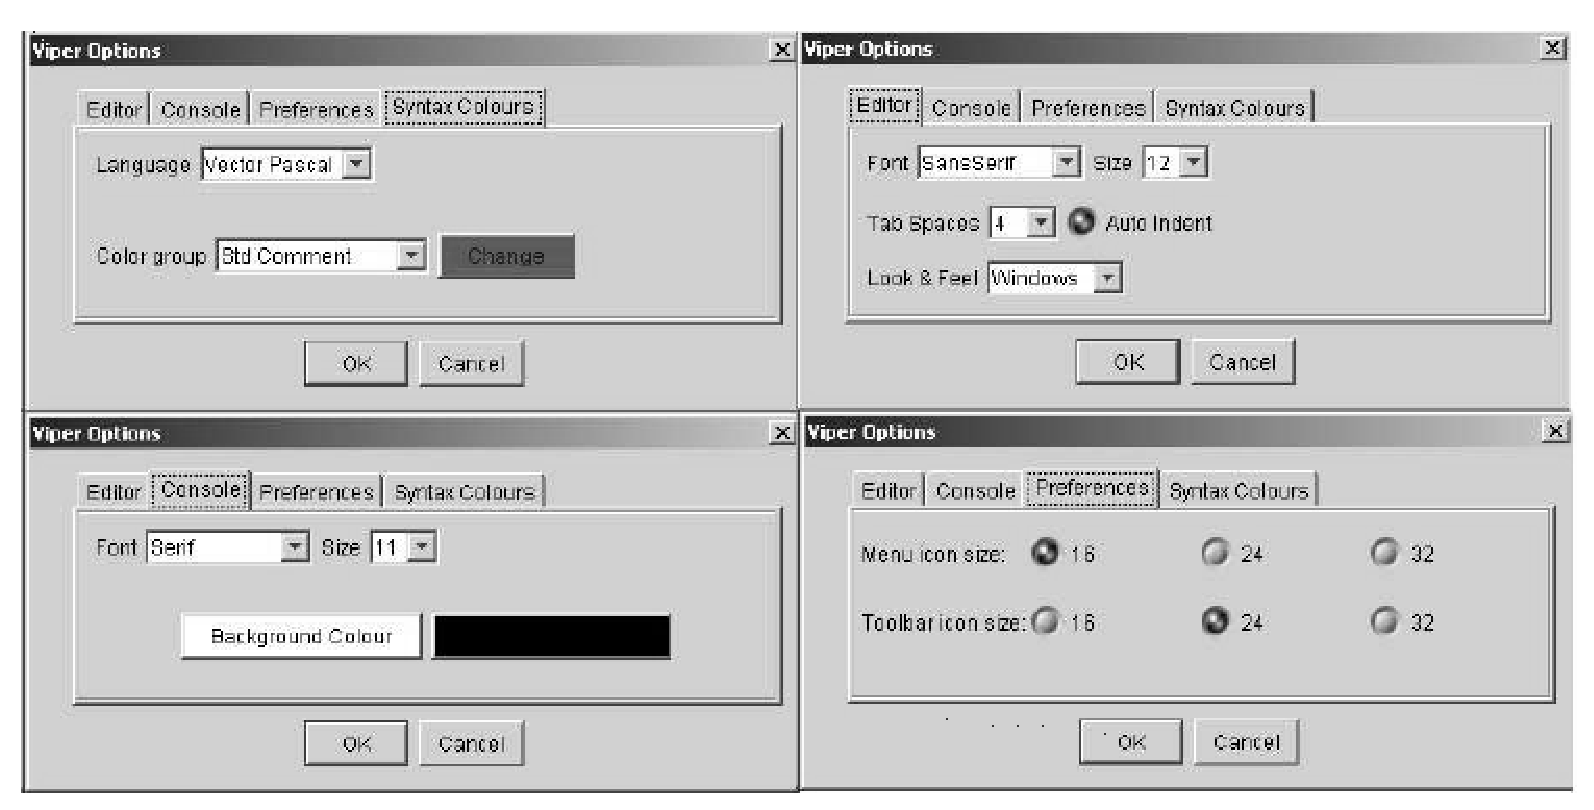
\epsfig{file=allviperoptions.eps,width=4.9in}
\caption{The Viper Option Windows}\label{fig:allvipops}
\end{figure}

The different Windows shown above allow the control of the VIPER I.D.E. The individual windows control:  -
\begin{itemize}
\item \textbf{Editor} This controls the look and feel (see Colour Plates) the font size and style, the tab size and auto indentation.
\item \textbf{Console} This controls the Font style and size and the background colour of the console window.
\item \textbf{Preferences} This allows the individual set-up of the menu icon sizes and the tool bar sizes.
\item \textbf{Syntax Colours} This allows the Syntax Highlighting colours to be altered to personal taste. These can be adjusted for each 
supported language (Vector Pascal, {\LaTeX}, HTML) independently.
\end{itemize}
\subsection{Dynamic Compiler Options}
\textbf{NOTE} This is for advanced use only.\\

This feature is intended to allow VIPER to handle: -
\begin{itemize}
\item  New processors as the class files become available (Dynamic class loading only).
\item New options for the compiler / new versions of the compiler.
\end{itemize}
The dynamically created options pages are added in the form of a new tabbed pane to the Compiler Options window.
To create a new options pane the user must: -
\begin{enumerate}
\item Open the file ../VectorPascal/viper/resources/dynamicOption.properties
\item Edit the file to suit the new options.
\item Save the  file.
\end{enumerate}
\subsubsection{Editing to add a processor}
In the file dynamicoptions.properties in the ../VectorPascal/viper/resources directory there is a list of the current processors.. This list  can be extended 
simply by adding another to the end of the list. It is best if the list ends with ``others''.

\textbf{Note}  The appropriate code generator files must be written for the Vector Pascal compiler and placed  in the ../VectorPascal/ilcg/tree  directory.
\subsubsection{Editing to add compiler options}
The dynamicoptions.properties file can be edited to produce a new compiler option. This is done by entering a new line at the end of the file following 
the in the line above. For example: -
\begin{figure}[h]
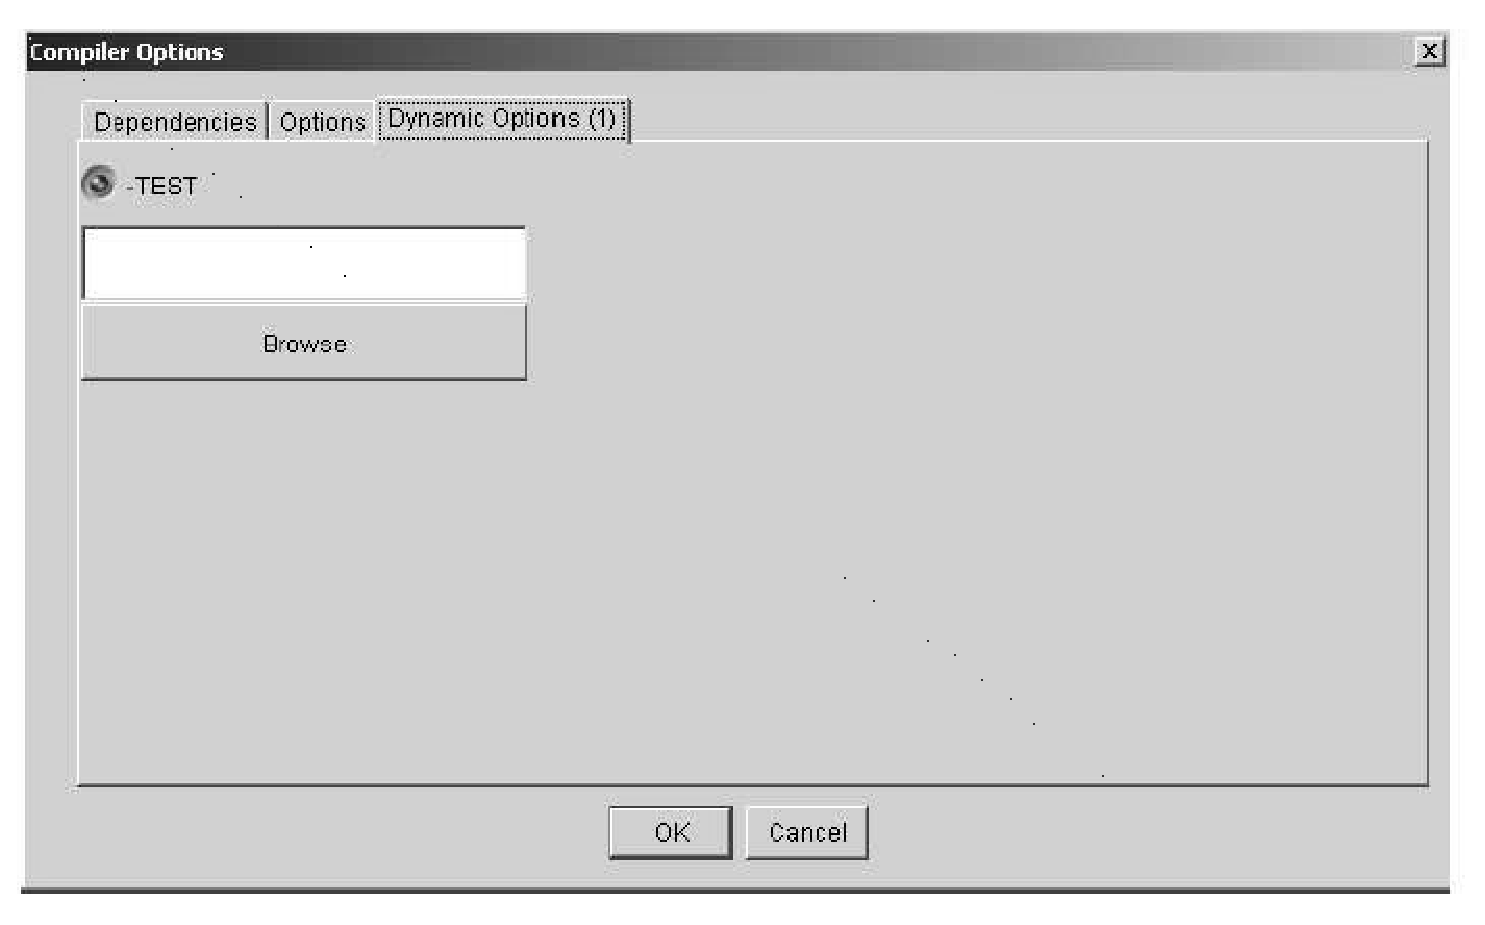
\epsfig{file=dynamicoptions.eps,width=4.5in}
\caption{Dynamic Option Window}\label{fig:DynamicOptions}
\end{figure}
\begin{verbatim}
CPUFLAGS: P3:K6:Pentium:IA32
#
#This is to set flags for the compiler
#NB DO NOT EDIT THIS FILE BEFORE AFTER READING THE HELP FILE
#IT IS IMPORTANT THAT THE FIELDS COME IN THE FOLLOWING ORDER
#FLAG(Type:String),DESCRIPTION(Type:String),TEXTFIELD(Type:int),
#BROWSEBUTTON(Type: boolean)
#Any comments must be but in this area.
		
FLAG:DESCRIPTION :TEXTFIELD: BROWSEBUTTON
-TEST:Test description: 20 : true:
\end{verbatim}

\subsection{VIPER Option Buttons}
The VIPER  options are set in their respective panels with the VIPER Option Buttons these have three states: -
\begin{itemize}
\item \textbf{Grey}  The item is  not selected.
\item \textbf{Red}  The mouse is over the correct areas to select the item.
\item \textbf{Blue}  The item is selected.
\end{itemize}

%%%%%%%%%%%%%%%%%%%%%%%%%%%%%%%%%%%%%%%%%%%%%%%%%%%%%%%%%%%%%%%%%%%%%%%%%%%%%%%%%%%%%%%%%%%%%%%%%%%%%%%%%%%%%%%%%%%%%%%%%%%

\section{Moving VIPER}
% author K.Renfrew

Ideally VIPER should be installed from the downloaded zip file on any new system. If this is not possible then it is still possible to move 
VIPER onto a new system even if the new host machine has a different operating system.

Moving a VIPER installation from any Windows host to any other Windows host, or from one Linux installation to another is 
straight forward.
\begin{enumerate}
\item Move the entire VectorPascal directory and all sub-directories to the new system.
\item Run VIPER and in the File menu click clear recent files and then click clear recent projects.
\item Import all projects that have been moved and are to be used on the new system.
\end{enumerate}
If the operating systems are  different (i.e. moving from Linux to Windows or vice versa) then the system must be reset: -
\begin{enumerate}
\item open a shell/DOS prompt window and change directories to the VectorPascal directory.
\item Type \texttt{ java ViperSystemReset} in the console window.
\end{enumerate}
The system is now reset and the new installation of VIPER can be used normally.

%%%%%%%%%%%%%%%%%%%%%%%%%%%%%%%%%%%%%%%%%%%%%%%%%%%%%%%%%%%%%%%%%%%%%%%%%%%%%%%%%%%%%%%%%%%%%%%%%%%%%%%%%%%%%%%%%%%%%%%%%%%
\section{Programming with VIPER}
% author K.Renfrew

This section assumes that the I.D.E. is now set-up to the user's taste. To open a file click the open file menu option and use the dialogue box to
open the file in the usual way. 

Familiarity with the basic editing functions of an I.D.E. are assumed.

%%%%%%%%%%%%%%%%%%%%%%%%%%%%%%%%%%%%%%%%%%%%%%%%%%%%%%%%%%%%%%%%%%%%%%%%%%%%%%%%%%%%%%%%%%%%%%%%%%%%%%%%%%%%%%%%%%%%%%%%%%%
\subsection{Single Files}
% author K.Renfrew

The file will open with the syntax highlighter associated with the file suffix of the target file. The file can be edited with all the usual I.D.E. functions.
(Cut, Paste, Copy, Save, Save As, Find and Replace, etc.).

VIPER features a ``right click menu'' to offer another method of quickly editing files.
\begin{figure}[h]\center
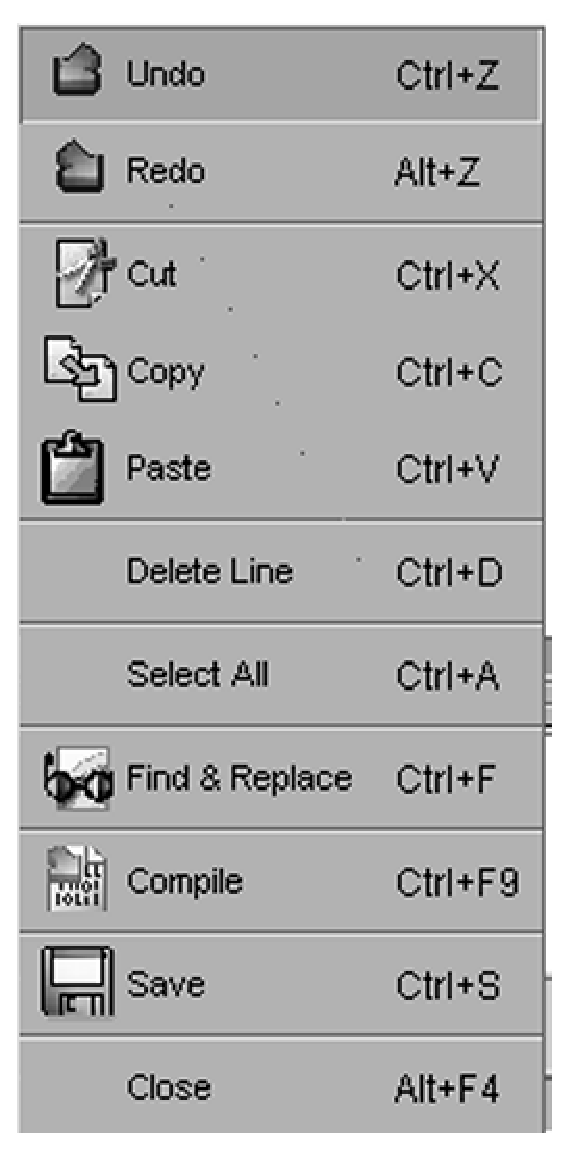
\epsfig{file=rightclick.eps,width=1.7in}
\caption{The Right Click Menu}\label{fig:rightclick}
\end{figure}

Line numbers can be viewed either by using the statistics on the status bar at the bottom right hand corner of the I.D.E. or by double clicking the dark grey 
panel on the left of the editor window, this line number panel can then be adjusted in size to suit the user's needs.

A new file can be opened from the file menu. Clicking on the New Document option allows the user to choose between the three types of file that  
VIPER supports (.Pascal, {\LaTeX}, HTML). A new file is then opened in the editor window. The file is un-named until it has been saved.

When a file has been changed since it was last saved the name tag at the top of the editor window appears in red, otherwise it is black.

If the user attempts to close the editor before a file is saved  the option to save the file is offered before the I.D.E. closes.

If a file has functions and / or procedures the function finder automatically displays these in the left  most editor window. Clicking on the icon 
by a function or procedure takes the editor to the start of that section.

%%%%%%%%%%%%%%%%%%%%%%%%%%%%%%%%%%%%%%%%%%%%%%%%%%%%%%%%%%%%%%%%%%%%%%%%%%%%%%%%%%%%%%%%%%%%%%%%%%%%%%%%%%%%%%%%%%%%%%%%%%%
\subsection{Projects}
% author K.Renfrew
The VIPER Project Manager allows the user to construct  software projects in Vector Pascal. 

An existing project can be opened using the Project / Open Project menu option or icon. The project will then appear in the project window.
The files names are in a tree structure which can be clicked to open the file in the editor window.

To create a new project the user clicks on the new project icon and the Project properties dialogue box will appear.
\begin{figure}[h]\center
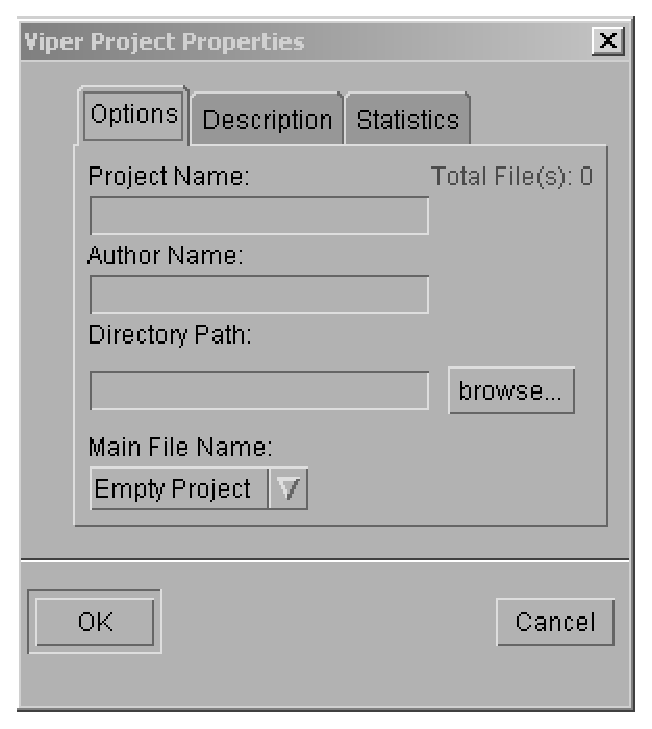
\epsfig{file=projprop.eps,width=3.0in}
\caption{The Project Properties Window}\label{fig:projprops}
\end{figure}

The text fields are then filled in to create the empty project. The directory path should be the parent directory for the project's  home directory.
This home directory will be given the project's name.

Once the project has been created the files can be added and removed as required.
\begin{itemize} 
\item \textbf{Adding} Click the add files icon and enter or browse for the required file. This copies the file to the project directory.
\item \textbf{Removing} Highlight the file too be removed and click the remove files icon. \textbf{Warning} This deletes the file from the project
directory.
\end{itemize}

Other files may be placed in the project directory but if they are not added to the project they will not be a member of the project.

The makefile for the project is automatically created as ProjectName.mke. The user should not edit either this or the .prj file directly.

\subsubsection{Importing Projects}
Projects can be imported from other VIPER installations by the import project facility. This can be found in Project / Import Project. Any project coming 
from another VIPER must be imported via this facility.

\subsubsection{Backing-Up Projects}
 The import project facility can be used to move an existing project to another directory of the same machine. This Back-Up project is not just a
 copy of the project but is fully functional with all the facilities of the VIPER system.

%%%%%%%%%%%%%%%%%%%%%%%%%%%%%%%%%%%%%%%%%%%%%%%%%%%%%%%%%%%%%%%%%%%%%%%%%%%%%%%%%%%%%%%%%%%%%%%%%%%%%%%%%%%%%%%%%%%%%%%%%%%
\subsection{Embedding {\LaTeX} in Vector Pascal}
% author K.Renfrew

The special comment (*! comment body *)  is used to embed {\LaTeX} in the Vector Pascal source file. Anything in within these comments will be treated 
as if it were {\LaTeX} both by the VP{\TeX}  system and the syntax highlighter. 

There is no need to put {\LaTeX}  commands in the special comments unless a specific result is required. (See section \ref{vptexstyle})
%%%%%%%%%%%%%%%%%%%%%%%%%%%%%%%%%%%%%%%%%%%%%%%%%%%%%%%%%%%%%%%%%%%%%%%%%%%%%%%%%%%%%%%%%%%%%%%%%%%%%%%%%%%%%%%%%%%%%%%%%%%
\section{Compiling Files in VIPER}
\subsection{Compiling Single Files}
% author K.Renfrew

Assuming the compiler has been set-up the compilation of a file is very simple. Simply click the compile icon (or menu option) and the compiler will
compile the file in the editor window with the options selected. 

The resulting files are placed in the same directory as the source file and are named the same as the source file with the corresponding suffix.

\subsubsection{Compiling a file to executable for several processors}

If a file is to be compiled for several different processors the CPUTAG and -CPU options must be set in the Set-Up / Compiler Options / Options panel.
The file MyProg.pas would then be compiled to ProcessorNameMyProg.exe.  This process can be done for each processor on the available processor 
list.

\textbf{Note}  A file compiled in this manner cannot be run within the I.D.E.

\subsection{Compiling Projects}
% author K.Renfrew

Projects can be compiled in two ways: -
\begin{itemize}
\item Make a project. This compiles the files that are not up to date but does not compile any file that is up to date.
\item Build a project.  This compiles all the files in the project regardless of whether the files are up to date.
\end{itemize}

The Vector Pascal compiler used in the traditional command line interface mode will check one level of dependency in a project. If there are more 
levels of dependency the VIPER project manager will automatically make a \texttt{makefile}  and recursively check all levels of  dependency in 
the project.

As VIPER compiles a file, the file is opened in the I.D.E. if an error is found compilation stops and the error is highlighted.
%%%%%%%%%%%%%%%%%%%%%%%%%%%%%%%%%%%%%%%%%%%%%%%%%%%%%%%%%%%%%%%%%%%%%%%%%%%%%%%%%%%%%%%%%%%%%%%%%%%%%%%%%%%%%%%%%%%%%%%%%%%
\section{Running Programs in VIPER}
% author K.Renfrew

\textbf{Note} Projects requiring input from the user \textbf{MUST} have the input redirected.

When a program has been compiled the resulting executable can be run in the I.D.E. by clicking on the Run icon. A redirect input box then appears.
If the program requires input from the user then an input file must be set. This file should contain all the data that the program requires to run to 
completion.

\begin{figure}[h]\center
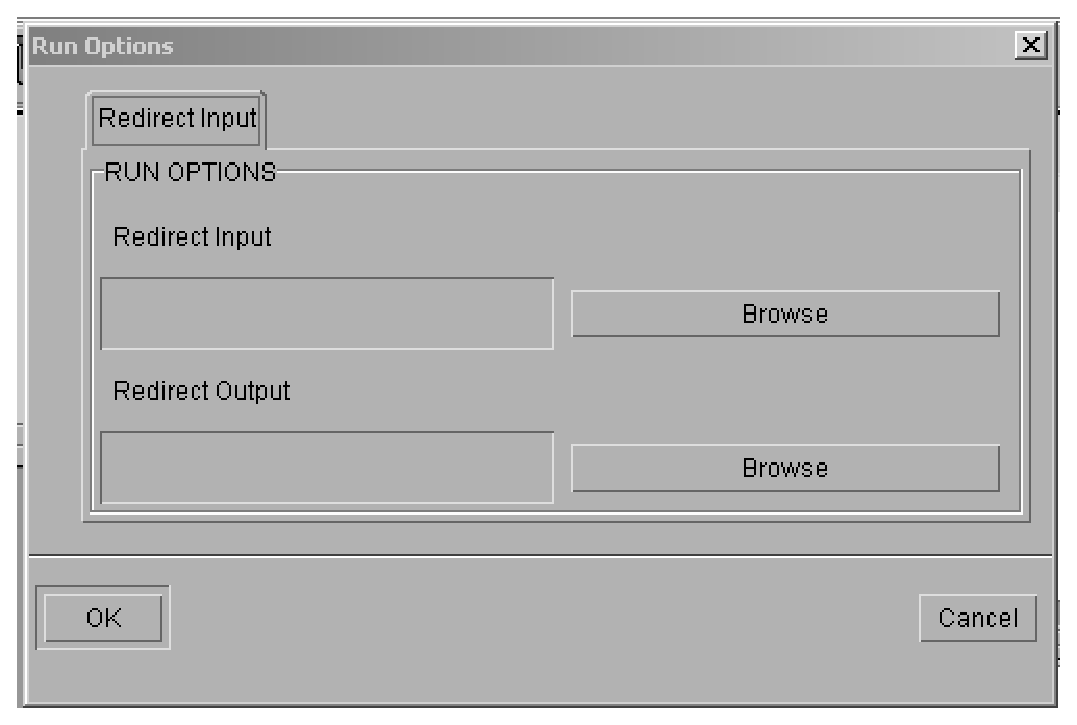
\epsfig{file=runops.eps,width=4.0in}
\caption{The Run Options Panel}\label{fig:run}
\end{figure}

Similarly the output may be redirected. This, however is not compulsory if the output is not redirected the output of the program appears in the console 
window. If the output is redirected then the output is written to the file set-up in the run dialogue window.


%%%%%%%%%%%%%%%%%%%%%%%%%%%%%%%%%%%%%%%%%%%%%%%%%%%%%%%%%%%%%%%%%%%%%%%%%%%%%%%%%%%%%%%%%%%%%%%%%%%%%%%%%%%%%%%%%%%%%%%%%%%
\section{Making VP{\TeX}}
% author K.Renfrew

Making VP{\TeX} is as simple as clicking the Build VP{\TeX}   icon or menu option. If  a project is open then the VP{\TeX}  is made for the whole 
project, otherwise the VP{\TeX} is made for the file in the editor window.

%%%%%%%%%%%%%%%%%%%%%%%%%%%%%%%%%%%%%%%%%%%%%%%%%%%%%%%%%%%%%%%%%%%%%%%%%%%%%%%%%%%%%%%%%%%%%%%%%%%%%%%%%%%%%%%%%%%%%%%%%%%
\subsection{VP{\TeX Options}}
% author K.Renfrew

The level of documentation is set by the user in the VP{\TeX} Options panel. This panel can be found in the TeX / VP-TeX Options menu item.
There are five levels of detail that can be chosen :-
\begin{itemize}
\item Function and Procedure headings only.
\item Level 1 plus all special comments.
\item Program bodies and interfaces.
\item Selected text
\item All source code.
\end{itemize}

In addition to the above options the user can choose whether a contents page is to be included or not. This is set by clicking the create contents page button.
 
\begin{figure}[h]\center
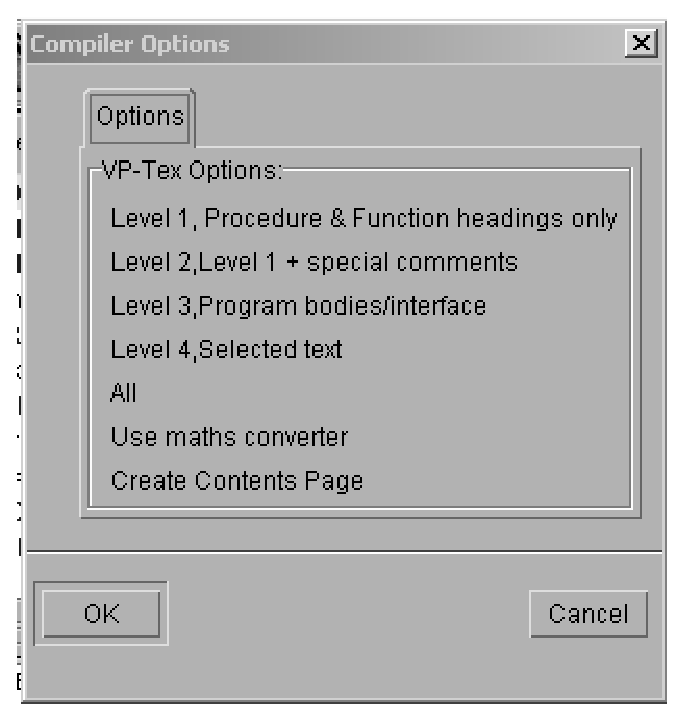
\epsfig{file=vptexoptions.eps,width=3.0in}
\caption{The VP{\TeX} Options Panel}\label{fig:texops}
\end{figure}
%%%%%%%%%%%%%%%%%%%%%%%%%%%%%%%%%%%%%%%%%%%%%%%%%%%%%%%%%%%%%%%%%%%%%%%%%%%%%%%%%%%%%%%%%%%%%%%%%%%%%%%%%%%%%%%%%%%%%%%%%%%
\subsection{VPMath}
% author K.Renfrew

The VPMath system converts Vector Pascal code to mathematical syntax. This makes the program more human readable and in general more concise.

The VPMath system is invoked automatically when the  VP{TeX}  is made if the Use Math Converter is set in the Tex/VP-TeX Options menu item.

%%%%%%%%%%%%%%%%%%%%%%%%%%%%%%%%%%%%%%%%%%%%%%%%%%%%%%%%%%%%%%%%%%%%%%%%%%%%%%%%%%%%%%%%%%%%%%%%%%%%%%%%%%%%%%%%%%%%%%%%%%%
\section{{\LaTeX}  in VIPER}
% author K.Renfrew

Most of the features of the VIPER editor used in the creation / editing of Vector Pascal files can also be used for creating / editing {\LaTeX} 
documents.

Opening a {\LaTeX}  document in VIPER automatically invokes the {\LaTeX} syntax highlighter and the Function Methods finder automatically 
changes to a Section /  Sub-Section finder. 

This allows the user to click on a Section icon in the left hand window and the editor will jump to that section.
  
%%%%%%%%%%%%%%%%%%%%%%%%%%%%%%%%%%%%%%%%%%%%%%%%%%%%%%%%%%%%%%%%%%%%%%%%%%%%%%%%%%%%%%%%%%%%%%%%%%%%%%%%%%%%%%%%%%%%%%%%%%%
\section{\texttt{HTML} in VIPER}
% author K.Renfrew

VIPER allows the user to edit/write HTML pages. The system for HTML is very straight forward. Create a new HTML file or open an existing file to be
edited. Once the file has been altered click on the run button just as if to run a Vector Pascal executable.

When a new HTML file is created or an existing one opened the HTML syntax highlighter is automatically loaded.

The default browser that is installed on the host machine will open with the HTML page displayed.

%%%%%%%%%%%%%%%%%%%%%%%%%%%%%%%%%%%%%%%%%%%%%%%%%%%%%%%%%%%%%%%%%%%%%%%%%%%%%%%%%%%%%%%%%%%%%%%%%%%%%%%%%%%%%%%%%%%%%%%%%%%
\section{Writing  Code to Generate Good VP{\TeX}} \label{vptexstyle}
% author 
%\subsection{Introduction to VP\TeX}
VPTeX is a tool included in the VIPER Integrated Development Environment for Vector Pascal.  It automatically produces and formats a LaTeX listing of the source file or files on which it is called.  By defining three distinct types of comments, VPTeX also allows the programmer to add extensive descriptions of their code to the listing, creating full LaTeX documentation for their Vector Pascal programs or projects.  Mathematical translation can also be performed on the source code listing to produce a more generic and succinct description of the program's algorithms and structures.

\paragraph{}The three types of comments available are:
\begin{description}
\item[Special Comments :]A special comment is started in the source code with the comment command (*! and terminated with *).  Special comments appear in the LaTeX as running prose and are of most use in giving extensive comments and descriptions of the program.  Special comments can include LaTeX commands, with some limitations, to further imrove the readability of the documentation.
\item[Margin Comments :]Normal Pascal \{...\} comments which appear immediately at the end of a line of code are placed in the left-hand margin adjacent to their source code line in the LaTeX documentation.  These are of principal use when a small description of the content of a single line is required.
\item[Normal Comments :]Normal Pascal \{...\} comments which appear on a line of their own will appear in the LaTeX in typewriter font.
\end{description}

\subsection{Use of Special Comments}
As outlined above, special comments are the principal means of describing a program in the documentation.  To maximise the effectiveness of the literate programming facility source code should be written with large amounts of special comments and with the program's documentation in mind.  The ability to include LaTeX command within special comments allows the programmer to directly affect the look of the LaTeX documentation, but there are some limits to the use of LaTeX commands within special comments:
\begin{itemize}
\item Do not include any preamble within special comments.  The preamble for the LaTeX documents is automatically produced by VPTeX.
\item Always use full text series altering commands such as \verb� \textbf{..}� rather than their shorthand equivalents such as \verb� \bf{...}�.
\item Bear in mind that any text entered in special comments must be compilable LaTeX for the documentation to compile.  This means that the following characters are control characters and should not be entered verbatim into special comments; \& \$ \% \_ \{ \} \^{} \~{} $\backslash$.
\end{itemize}

\paragraph{}
Special comments can be particularly useful for controlling the structure of your LaTeX document.  The following are guidelines as to how to structure your documentation.
\begin{itemize}
\item For an individual program or unit file, the LaTeX document produced by VPTeX will be an article, so sections are the highest level description that can be applied to a block of text.
\item It is usually useful to include an introduction to the program at the start of the Pascal source file using the \verb�\section{Introduction}� comand at the start of an opening special comment.
\item A special comment containing just a structure command (\verb�\section, \subsection� etc.) can be extremely useful in sectioning off different parts of the source code to add structure to the code listing.  For example, the declarations could be prefaced with \verb�(*! \section{Declarations} *)� or the main program could be prefaced with a similar command.  Each procedure or function is automatically placed within its own section by VPTeX so do not add structuring special comments to these sections of code.
\end{itemize}

\paragraph{}
To produce a well documented program, it is important that special comments are regularly employed to add verbose descriptions of the source code.  It is not uncommon for a LaTeX documentation file to contain many pages of special comments split into sections and subsections between small sections of code.  VPTeX also automatically creates a content page so the structure of your special comments will be reflected in the content page.

\paragraph{}
Note: With the current release of the Vector Pascal compiler, special comments containing *'s other than at the opening (*! and closing *) tags will not compile.

\subsection{Use of Margin Comments}
Margin comments are useful for providing short descriptions of the purpose of individual lines of code.  If the meaning of a particular code line is especially cryptic, or the significance of the line needs to be emphasised, a  margin comment stating the purpose of that line may be useful.  Please be aware that because margin comments necessarily reside in the left-hand margin of the finished document, lengthy comments will spill onto many lines and break up the flow of the code.  It is advised that margin comments should not be more than 10 or so words, with the other types of comments available if a longer description is required.

\paragraph{}
The VPTeX tool automatically breaks lines following the \textsf{\textbf{var}} and \textsf{\textbf{const}} keywords. Therefore, the declaration following these keywords will be placed on a new line, but any margin comment for this line will not.  It is recommended that the programmer takes a new line after the \textsf{\textbf{var}} and \textsf{\textbf{const}} keywords.

\subsection{Use of Ordinary Pascal Comments}
The function of normal Pascal comments has been superceded in most cases by VPTeX's Special Comments.  However, normal comments can still be useful in a number of circumstances.  The following list details the recommended usage of normal Pascal comments, but the user is, of course, free to make use of them in any circumstances he wishes.
\begin{itemize}
\item Firstly, because normal comments are displayed in typewriter font, any spacing within these comments set out by the programmer will be preserved in the documentation.  This is not the case for special comments which are displayed in a serifed, variable width font.  This property of normal comments makes them particulary suitable for laying out tables and arrays simply, although a special comment can make use of LaTeX's ability to typeset tables for a more advanced layout.
\item Secondly, normal comments do not break up the flow of a code listing to the same extent as special comments and so are more useful for offering a running commentary on code lines, without the space limitations of margin comments.
\item If a comment is reasonably short, the programmer may find that a normal comment will have a better appearance than a special comment. Since special comment are offset from the program listing a small special comment may constitute a waste of the space set aside for it.
\end{itemize}

\subsection{Levels of Detail within Documentation}
Depending on the sort of documentation you want to produce, VPTeX allows the programmer to specify the detail of their program documentation.  The five levels are:
\begin{enumerate}
\item \textbf{Procedure and Function Headings Only:} For documentation of ADT's it is often useful to simply provide a list of the functions and procedures by which a programmer may make use of the ADT.  VPTeX supports this by providing the option to create documentation consisting of only function and procedure headings.  It is advised that a contents page is not included with this level of detail.
\item \textbf{Special Comments with Function and Procedure Headings:} To add commentary and descriptions to the above level of detail, option 2 will add any special comments to the documentation.  This allows the programmer to provide descriptions of their procedures and functions and to add structure to the documentation.  A contents page is advised for this level of detail.
\item \textbf{Program Bodies and Unit Interfaces:} This level of detail includes all comments.  It is again very useful for documenting ADT's as the interfaces provided by units will be documented, but none of the implementation will be included.  A contents page is recommended.
\item \textbf{Selected Text:} Special VPTeX comments commands have been defined to allow the programmer to select which sections of their program to document. The commands are \texttt{(*!begin*)} to mark the start of a selected region, and \texttt{(*!end*)} to mark the end.  Any text, including special comments, not contained within these tags will be ignored by VPTeX if this level of detail is selected.  The start and end of the main program file will always be included in the documentation regardless of selection.  This feature is of particular use when preparing reports regarding particular sections of code within long projects as only the sections of interest will be documented.  Again, a contents page is recommended.
\item \textbf{All Code and Comments:} For a completely documented code listing, of particular use for system maintenance, VPTeX can produce a complete listing of a program or project's source code, including special and normal comments.  A contents page is strongly recommended, particularly for long programs or projects.
\end{enumerate}
Note: All levels of detail support margin comments.

\subsection{Mathematical Translation: Motivation and Guidelines}
VPTeX has the option of automatically translating the program code into conventional mathematical notation.
Complex VectorPascal expressions like:\\ \\
myVariable:= if (iota 0 div 2 pow (dim-iota 1)) mod 2 = 0 then 1 else -1;\\ \\
are translated into more tidy and comprehensible mathematical representations like.\\ \\
\textsf{$\textit{myVariable}\leftarrow \left\{ \begin{array}{ll}
       1 & \mbox{if ($\frac{\iota_{ 0 }}{2^{dim - \iota_{ 1 }}}$)\textbf{ mod }2 $=$ 0}\\
        -  1 & \mbox{otherwise}\\
\end{array} \right.$};\\ \\
No action is required to get mathematical translation, so long as it is turned on (VP-TeX Options),
however the benefits of using it increse with the number of mathematical structures in the document.
In particular, the following will benefit from mathematical translation:
\begin{itemize}
\item{Array indexing/slicing, e.g thisArray$_{i,j}$ / thatArray$_{low..high}$}
\item{Assignments, e.g. myVarable $\leftarrow$ yourVariable}
\item{Reduction operations on arrays, e.g myVariable $\leftarrow$ $\sum$oneDArray}
\item{Conditional updates (as shown above)}
\item{A number of standard mathematical function such as $\sqrt{\ \ }$}
\item{Mathematical operations, e.g. x$^y$,  $\frac{a}{b}$, $i \times j$}
\item{English names of Greek letters (lower case only), e.g. $\alpha$, $\beta$, $\gamma$, $\delta$}
\end{itemize}
Mathematical translation is particularly useful if the documentation is for people without knowledge of Pascal or a similar language.
The only time mathematical translation is not advisable is when the reader is maintaining the code itself,
in which case the need for cross reference will usually dominate the need for clarity and conventional notation.

\subsection{LaTeX Packages}
All VPTeX documents only include packages \texttt{graphicx} and \texttt{epsfig}.  
These packages are included to allow the programmer to include graphics and 
diagrams to help document their programs.  Any LaTeX commands the programmer
 may wish to use which are specific to other packages cannot be included in 
VPTeX special comments.


%%%%%%%%%%%%%%%%%%%%%%%%%%%%%%%%%%%%%%%%%%%%%%%%%%%%%%%%%%%%%%%%%%%%%%%%%%%%%%%%%%%%%%%%%%%%%%%%%%%%%%%%%%%%%%%%%%%%%%%%%%%

%\end{document}

